% Created 2024-09-04 Wed 15:25
% Intended LaTeX compiler: pdflatex
\documentclass[letterpaper, 12pt]{article}
\usepackage[utf8]{inputenc}
\usepackage[T1]{fontenc}
\usepackage{graphicx}
\usepackage{longtable}
\usepackage{wrapfig}
\usepackage{rotating}
\usepackage[normalem]{ulem}
\usepackage{amsmath}
\usepackage{amssymb}
\usepackage{capt-of}
\usepackage{hyperref}
\usepackage{minted}
\usepackage{xcolor}
\usepackage{hyperref}
\usepackage{tocloft}
\usepackage{minted}
\usemintedstyle{manni}
\usepackage{pdfpages}
\usepackage{fancyhdr}
\usepackage{graphicx}
\usepackage[top=1.4in, left=0.5in, right=0.5in, bottom=0.8in]{geometry}
\usepackage[T1]{fontenc}
\usepackage{helvet}
\pagestyle{fancy}
\renewcommand{\headrulewidth}{0pt}
\renewcommand{\footrulewidth}{0pt}
\setlength{\parindent}{0em}
\setlength{\parskip}{1em}
\usepackage{hyperref}
\usepackage {color}
\usepackage {tabularray}
\usepackage{xcolor}
\hypersetup{
colorlinks=true,
linkcolor=blue,
filecolor=magenta,
urlcolor=cyan,
citecolor=green,
pdfborder={0 0 0}
}
\usepackage[most]{tcolorbox}
\author{Hilduara Abreu}
\date{\today}
\title{PS192 | Cartas de Bienvenida Año Académico 2024-25\\\medskip
\large Versión en Español}
\hypersetup{
 pdfauthor={Hilduara Abreu},
 pdftitle={PS192 | Cartas de Bienvenida Año Académico 2024-25},
 pdfkeywords={},
 pdfsubject={},
 pdfcreator={Emacs 29.4 (Org mode 9.6.15)}, 
 pdflang={English}}
\begin{document}


\includepdf[pages=1,fitpaper]{/home/rob/.ps192_welcome_letters/Welcome-Year-2024/welcome-letters/pdf1.pdf}

\fancyfoot[C]{\setlength{\unitlength}{1in}\begin{picture}(5,0)\put(-1.8,-0.5){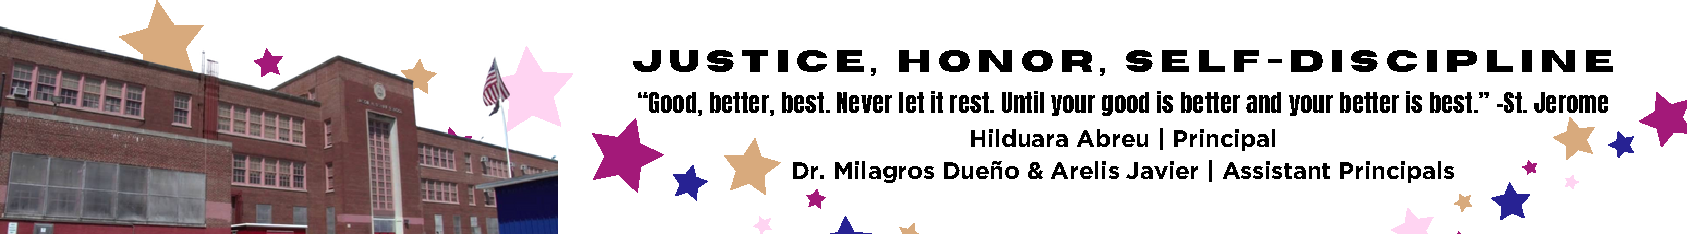
\includegraphics[width=8.8in,height=1.3in]{logo-1}}\end{picture}}
\fancyhead[C]{\setlength{\unitlength}{1in}\begin{picture}(5,0)\put(-1.9,-0.5){
\includegraphics[width=8.9in,height=1.3in]{logo-2}}\end{picture}}
\fancyhead[R]{\thepage}
\pagenumbering{gobble}

\begin{document}
\newpage
\vspace*{-0.5cm}

\section*{Tabla de Contenidos}
\label{sec:orga9abbca}
\begin{itemize}
\item \hyperref[sec:orgcbc1d4c]{Introducción}
\item \hyperref[sec:org9f0a792]{Horario Escolar}
\item \hyperref[sec:org88a530b]{Política de Uniformes}
\item \hyperref[sec:orga396db2]{Uso de Dispositivos Electrónicos}
\item \hyperref[sec:orgb5585fa]{Carta de Bienvenida 3-K y Pre-K}
\item \hyperref[sec:org5f07f09]{Carta de Bienvenida Grados K-5}
\item \hyperref[sec:org22c5294]{Criterios de Promoción y Política de Calificaciones}
\end{itemize}

\newpage
\vspace*{-0.5cm}

\tcbuselibrary{}
\newtcolorbox{bluebox}[1][]{
  colback=blue!5!white,
  colframe=blue!75!black,
  fonttitle=\bfseries,
  coltitle=black,
  enhanced,
  attach boxed title to top center={yshift=-2mm},
  title=#1,
  boxed title style={colback=blue!50!white}
}
\newtcolorbox{greenbox}[1][]{
  colback=green!5!white,
  colframe=green!75!black,
  fonttitle=\bfseries,
  coltitle=black,
  enhanced,
  attach boxed title to top center={yshift=-2mm},
  title=#1,
  boxed title style={colback=green!50!white}
}
\newtcolorbox{redbox}[1][]{
  colback=red!5!white,
  colframe=red!75!black,
  fonttitle=\bfseries,
  coltitle=black,
  enhanced,
  attach boxed title to top center={yshift=-2mm},
  title=#1,
  boxed title style={colback=red!50!white}
}

\section*{Introducción}
\label{sec:orgcbc1d4c}
Estimado Padre o Tutor,

¡Bienvenido a PS 192! Estamos comprometidos en proporcionar un ambiente seguro y acogedor donde cada estudiante pueda prosperar académicamente, socialmente y emocionalmente. A medida que iniciamos otro emocionante año escolar, es esencial que todos los miembros de nuestra comunidad escolar se mantengan informados sobre nuestras políticas, reglas, eventos y valores fundamentales. Estas directrices nos ayudan a crear un ambiente de aprendizaje positivo y productivo para nuestros estudiantes.

\begin{quote}
"La educación es el viaje donde la Justicia, el Honor y la Auto-disciplina nos guían para desbloquear nuestro máximo potencial. En PS 192, creemos en cultivar estos valores fundamentales para inspirar grandeza en cada estudiante, padre y maestro, sentando las bases para un futuro más brillante. Juntos, emprendamos este nuevo año académico con un compromiso compartido con la excelencia y una pasión por el aprendizaje continuo."   -- Hilduara Abreu
\end{quote}

En PS 192, creemos en el poder de la educación para transformar vidas. Nuestro personal dedicado trabaja incansablemente para ofrecer la más alta calidad educativa, empoderando a nuestros estudiantes para que se conviertan en la próxima generación de pensadores y líderes que tendrán un impacto positivo en nuestra ciudad y más allá. Su asociación y apoyo son cruciales en este viaje, y les agradecemos por ser una parte integral de nuestra comunidad.

Juntos, podemos asegurar que PS 192 continúe siendo un lugar donde cada niño se sienta valorado e inspirado para alcanzar su máximo potencial. Esperamos un año escolar exitoso y enriquecedor con su continua participación y cooperación.

Con justicia, honor y autodisciplina,


\includegraphics[width=0.2\textwidth]{hil_signature}

\textbf{Hilduara Abreu, Principal}

\textit{¡La Escuela del Aprendizaje Alegre!}

\href{www.ps192.org}{www.ps192.org}
\pagebreak
\vspace*{-1cm}

\subsection*{Horario Escolar}
\label{sec:org9f0a792}
Estimado Padre o Tutor,

Un horario escolar especifica la hora de inicio y duración de uno o más períodos de instrucción cada día. Un horario diario consistente y rutinas paso a paso proporcionan a los niños un día predecible. Un Horario Escolar ayuda a los niños a:
\begin{itemize}
\item Sentirse en control de su entorno
\item Sentirse seguros y cómodos
\item Saber qué está sucediendo ahora y qué viene después
\item Saber cómo realizar una actividad o tarea
\item Participar en el aprendizaje
\end{itemize}

Al igual que los adultos, los niños se sienten más confiados y seguros cuando sus actividades diarias son predecibles y familiares.

\begin{bluebox}[PS 192 | Horario Escolar]
\begin{table}[H]
\centering
\begin{tblr}{
  colspec={|X|X|X|X|},
  row{1}={font=\bfseries\color{MacaroniandCheese},c},
  hlines,
  vlines,
  hline{1,10} = {-}{0.08em},
}
\textbf{Período} & \textbf{Hora de Inicio} & \textbf{Hora de Fin} & \textbf{Duración} \\
1               & 08:00 AM            & 08:45 AM          & 45 minutos      \\
2               & 08:45 AM            & 09:30 AM          & 45 minutos      \\
3               & 09:30 AM            & 10:15 AM          & 45 minutos      \\
4               & 10:15 AM            & 11:05 AM          & 50 minutos      \\
5               & 11:05 AM            & 11:55 AM          & 50 minutos      \\
6               & 11:55 AM            & 12:40 PM          & 45 minutos      \\
7               & 12:40 PM            & 01:30 PM          & 50 minutos      \\
8               & 01:30 PM            & 02:15 PM          & 45 minutos
\end{tblr}
\end{table}
\end{bluebox}

\pagebreak
\vspace*{-0.5cm}

\textbf{Notas}:
\begin{itemize}
\item La puntualidad es crucial para un inicio suave del día. Por favor, asegúrese de que su hijo llegue a tiempo para aprovechar al máximo cada día escolar.
\item Las interrupciones durante el horario de clases deben ser mínimas para asegurar la mejor experiencia de aprendizaje posible para todos los estudiantes.
\end{itemize}

Por favor, mantenga una copia del horario escolar para su referencia y ayúdenos a apoyar a sus hijos para que se beneficien al máximo de su tiempo en PS 192.

Con justicia, honor y autodisciplina,


\includegraphics[width=0.2\textwidth]{hil_signature}

\textbf{Hilduara Abreu, Principal}

\textit{¡La Escuela del Aprendizaje Alegre!}

\href{www.ps192.org}{www.ps192.org}
\pagebreak
\vspace*{-1cm}

\subsection*{Política de Uniformes}
\label{sec:org88a530b}
Estimado Padre o Tutor,

La política de uniformes se aplicará durante el horario escolar y en todos los eventos y actividades relacionadas con la escuela, como excursiones y asambleas especiales.

\begin{enumerate}
\item \textbf{Camisa Burdeos}: Todos los estudiantes deben usar una camisa de color burdeos como parte superior del uniforme.
\item \textbf{Pantalones Azules}: Se deben usar pantalones o pantalones cortos de color azul marino como parte inferior del uniforme.
\end{enumerate}

\textbf{\textbf{Beneficios de la Política de Uniformes}}

Los uniformes sirven como un elemento unificador dentro de nuestra comunidad escolar y ofrecen varias ventajas significativas:

\begin{enumerate}
\item \textbf{Promoción de la Igualdad}: Los uniformes eliminan las disparidades socioeconómicas entre los estudiantes, asegurando que todos estén vestidos de la misma manera, independientemente de las circunstancias financieras de sus familias.
\item \textbf{Mejora del Enfoque}: Usar uniformes reduce las distracciones relacionadas con la moda y la presión de los compañeros, permitiendo que los estudiantes se concentren en sus estudios y crecimiento personal.
\item \textbf{Fomento del Orgullo Escolar}: Un uniforme infunde un sentido de orgullo y pertenencia entre los estudiantes, ayudándolos a identificarse y apreciar su comunidad escolar.
\item \textbf{Mejora de la Seguridad}: Los uniformes facilitan la identificación de intrusos en las instalaciones escolares, mejorando la seguridad general.
\item \textbf{Preparación para el Éxito Futuro}: Fomentar un código de vestimenta similar a la vestimenta profesional ayuda a preparar a los estudiantes para futuras carreras en las que una apariencia profesional es importante.
\end{enumerate}

\textbf{\textbf{Días de Vestimenta Casual}}

Entendemos que la expresión personal es importante y, por lo tanto, se programarán ocasionalmente "Días de Vestimenta Casual" a lo largo del año escolar, permitiendo a los estudiantes expresar su individualidad \newpage \vspace*{-0.5cm} a través de sus elecciones de ropa. Solicitamos amablemente su cooperación y apoyo para garantizar que su hijo llegue a la escuela vestido de acuerdo con nuestra política de uniformes. Creemos que esto contribuirá a un entorno de aprendizaje más positivo y productivo para todos los estudiantes.

\textbf{\textbf{Información de Contacto}}

Si tiene alguna pregunta o inquietud respecto a la política de uniformes, no dude en comunicarse con nuestra Coordinadora de Padres, Sra. Angela Rijo, a través de los siguientes canales:
\begin{itemize}
\item Sitio web: \url{https://www.ps192.org/angela}
\item Grupo de Whatsapp
\item ClassDojo
\item Teléfono: (212) 775-9560
\item En persona durante el horario de oficina: 9:00 AM - 3:00 PM
\end{itemize}

Estamos aquí para asistirle y apoyarle.

\textbf{\textbf{Cierre}}

Gracias por su colaboración en el fortalecimiento de una comunidad de aprendizaje fuerte y vibrante en PS 192. Esperamos un año académico exitoso y enriquecedor.

Con Justicia, Honor y Auto-disciplina,


\includegraphics[width=0.2\textwidth]{hil_signature}

\textbf{Hilduara Abreu, Directora}

\textit{¡La Escuela del Aprendizaje Alegre!}

\href{https://www.ps192.org}{www.ps192.org}

\pagebreak
\vspace*{-1cm}

\subsection*{Uso de Dispositivos Electrónicos}
\label{sec:orga396db2}
Estimado Padre o Tutor,

\begin{redbox}[PS 192 | Dispositivos Prohibidos]
Aunque no se recomienda, se permite a los estudiantes llevar los siguientes dispositivos electrónicos a la escuela:
\begin{itemize}
\item Teléfonos móviles
\item Sistemas portátiles de música y entretenimiento (por ejemplo, iPods, reproductores de MP3)
\end{itemize}
\textit{El estudiante y/o el padre es responsable de la seguridad y protección de estos dispositivos. La escuela no proporciona instalaciones para cargar los dispositivos.}
\vspace*{3mm}

Puntos Clave Importantes:
\begin{itemize}
\item Antes de las 8:00 AM o después de las 3:35 PM en cualquier lugar dentro de la escuela donde no interrumpa las actividades educativas.
\item Deben estar apagados o no utilizados durante el tiempo de instrucción, excepto para fines educativos con la aprobación del maestro.
\item Deben estar apagados o no utilizados durante cuestionarios, exámenes o pruebas a menos que se autorice explícitamente o sea parte de un Programa de Educación Individualizada (IEP) o Plan de Adaptación Sección 504.
\item Deben estar en posesión de los estudiantes durante el horario de campana de la escuela.
\item Deben estar apagados o no utilizados durante simulacros de incendio u otros ejercicios de preparación para emergencias.
\item No deben usarse en los baños.
\item No deben usarse durante el almuerzo en la cafetería o en el patio escolar.
\item No deben usarse entre clases en pasillos y escaleras.
\end{itemize}
\end{redbox}
\newpage \vspace*{-0.5cm}
El uso de dispositivos electrónicos debe cumplir con el Código de Disciplina del DOE, la política escolar, la Regulación del Canciller A-413 y la Política de Uso y Seguridad Aceptable de Internet (IAUSP) del DOE.

Con Justicia, Honor y Auto-disciplina,


\includegraphics[width=0.2\textwidth]{hil_signature}

\textbf{Hilduara Abreu}, \textbf{Directora}

\textit{¡La Escuela del Aprendizaje Alegre!}

\href{https://www.ps192.org}{www.ps192.org}

\pagebreak
\vspace*{-1cm}

\subsection*{Carta de Bienvenida 3-K y Pre-K}
\label{sec:orgb5585fa}
Estimado Padre o Tutor,

¡Estamos contando los días hasta la llegada de nuestros estudiantes el jueves, 5 de septiembre de 2024! Nuestros dedicados instructores y el personal escolar están ansiosos por darles la bienvenida a lo que promete ser un año emocionante de fomentar conexiones y construir una comunidad sólida. Nuestros cariñosos educadores están emocionados de compartir su risa, energía y pasión por el aprendizaje con sus hijos.

A medida que nos preparamos para el regreso de su hijo, queremos compartir información importante que se encuentra en P.S. 192 para asegurar una experiencia de aprendizaje segura y agradable para todos. Por favor, tome nota de las siguientes pautas:
\begin{redbox}[PS 192 | ¡Puntos Clave para Mejorar el Aprendizaje!]
\begin{itemize}
\item Uniformes: Todos los estudiantes deben asistir a la escuela diariamente con su uniforme, que sigue siendo el mismo: una camiseta burdeos y pantalones o falda azul marino (pantalones, falda, jumper).
\item Llegada y Salida: Para garantizar un proceso de llegada y salida seguro y eficiente, por favor tome nota del siguiente horario. Habrá miembros del personal y señales que indicarán a las familias dónde deben ir durante la primera semana de clases.
  \begin{itemize}
  \item Llegada: Patio trasero a las 8:00 AM
  \item Salida: Patio trasero a las 2:15 PM
  \end{itemize}
\item Primeros Días de Escuela: Aunque todos los estudiantes tendrán un horario escolar de 8:00 AM a 2:20 PM cada día, se invita a los padres a permanecer con sus hijos el jueves y viernes de 8:00 AM a 10:00 AM para ayudar a nuestros jóvenes estudiantes a adaptarse al entorno escolar.
\item Materiales Escolares: P.S. 192 proporcionará todos los materiales escolares básicos, como cuadernos, carpetas y crayones. Solo pedimos que las familias de 3K y PreK proporcionen una mochila, ropa de cambio y materiales para su tiempo de siesta diaria (mantita, sábana y/o un objeto de transición pequeño como una muñeca o peluche).
\end{itemize}
\end{redbox}
Nos sentimos privilegiados de ser parte de una comunidad donde padres, maestros, personal y estudiantes trabajan juntos para construir relaciones sólidas que apoyen el crecimiento académico y social. Estamos ansiosos por su participación en los diversos eventos a lo largo del año escolar y les damos la bienvenida a su participación activa en el viaje educativo de su hijo.
\newpage \vspace*{-0.5cm}
Actualizaciones regulares sobre eventos escolares se comunicarán a través de nuestro sitio web: \href{https://www.ps192.org}{www.ps192.org}, \href{https://www.classdojo.com/}{ClassDojo}, School Messenger y nuestro grupo de WhatsApp. Si tiene alguna pregunta, no dude en contactar a nuestra Coordinadora de Padres, Angela Rijo, a \href{mailto:arijo@schools.nyc.gov}{arijo@schools.nyc.gov}, sitio web escolar: \href{https://www.ps192.org/angela}{www.ps192.org/angela}, o al (212) 775-9560.

Estaremos organizando eventos a lo largo del año y esperamos asociarnos con ustedes tanto en persona como virtualmente. Por favor, manténgase atento a más información sobre todos nuestros eventos próximos:
\begin{itemize}
\item El 12 de septiembre, estaremos organizando Conferencias de Padres y Maestros por la Noche.
\end{itemize}

Estamos emocionados de comenzar este año escolar y colaborar con ustedes para asegurar que su hijo disfrute de la mejor experiencia de aprendizaje posible—una en la que se sientan valorados, alentados y emocionados por aprender y sus posibilidades ilimitadas.

Me siento profundamente honrada de servir como directora de PS 192. Gracias por su cooperación inquebrantable y dedicación a nuestros estudiantes, personal y facultad. Espero colaborar con ustedes en el viaje educativo de su hijo.

Con Justicia, Honor y Autodisciplina,


\includegraphics[width=0.2\textwidth]{hil_signature}

\textbf{Hilduara Abreu, Directora}

\textit{¡La Escuela del Aprendizaje Alegre!}

\href{www.ps192.org}{www.ps192.org}
\pagebreak
\vspace*{-1cm}

\subsection*{Carta de Bienvenida Grados K-5 2024}
\label{sec:org5f07f09}
Estimado Padre o Tutor,

A medida que se acerca el inicio del nuevo año escolar 2024-25, que comenzará el 5 de septiembre, les extendemos una cálida bienvenida a todos nuestros estudiantes. Esperamos que hayan tenido unas vacaciones de verano agradables y saludables. Nuestro dedicado y compasivo equipo de educadores y personal escolar espera con ansias su regreso para lo que promete ser un año lleno de emoción, risas y aprendizaje.

\begin{greenbox}[PS 192 | ¡Puntos Clave para Mejorar el Aprendizaje!]
\begin{itemize}
\item Uniformes: Todos los estudiantes deben asistir a la escuela diariamente vestidos con sus uniformes, que permanecen igual: una camiseta burdeos y pantalones o falda azul marino (pantalones, falda, overol).
\item Llegada y Salida: Para garantizar un proceso de llegada y salida seguro y eficiente, tome nota del siguiente horario. Habrá miembros del personal y señales que guiarán a las familias durante la primera semaElp
\item Llegada: Este año, TODOS los estudiantes de los grados K-5 ingresarán a través de la Cafetería cada mañana, a partir de las 7:40 AM para desayunar.
\item Salida: Este año, TODOS los estudiantes de los grados K-5 serán despedidos desde el patio trasero a las 2:15 PM. Habrá lugares designados para cada clase por grado. Por favor, siga las señales.
\item Suministros Escolares: PS 192 proporcionará todos los suministros escolares básicos, como cuadernos, carpetas y crayones. Solo pedimos que las familias de los grados K-5 proporcionen a los estudiantes una mochila y una caja de bolsas Ziplock tamaño galón para que los estudiantes las utilicen en los centros, mochilas y kits de herramientas matemáticas.
\end{itemize}
\end{greenbox}

\subsubsection*{Comunidad y Eventos}
\label{sec:orgdd43da3}
Nos sentimos privilegiados de ser parte de una comunidad donde padres, maestros, personal y estudiantes trabajan juntos para construir relaciones sólidas que apoyen el crecimiento académico y social. Estamos ansiosos por su participación en los diversos eventos a lo largo del año escolar y valoramos su participación activa en el viaje educativo de su hijo. Es un honor formar parte de una comunidad en la que padres, maestros, personal y estudiantes trabajan en conjunto para fomentar relaciones sólidas que promuevan el crecimiento académico y social. Esperamos con entusiasmo su participación en los eventos programados a lo largo del año escolar y apreciamos su compromiso activo en la educación de su hijo.

Las actualizaciones regulares sobre los eventos escolares de su hijo se comunicarán a través de nuestro sitio web: \newpage \vspace*{-0.5cm} \href{http://www.ps192.org}{www.ps192.org}, ClassDojo, School Messenger y nuestro grupo de WhatsApp. Si tiene alguna pregunta, no dude en contactar a nuestra Coordinadora de Padres, Angela Rijo, en \href{http://www.ps192.org/angela}{www.ps192.org/angela}, o al (212) 775-9560.

Estaremos organizando eventos a lo largo del año y esperamos asociarnos con ustedes tanto en persona como virtualmente. Por favor, esté atento a más información sobre todos nuestros próximos eventos:

\textbf{Evento Próximo}
\begin{itemize}
\item El 12 de septiembre, estaremos organizando nuestras Conferencias de Padres y Maestros por la Noche.
\end{itemize}

Estamos contando los días hasta poder darles la bienvenida nuevamente el jueves 5 de septiembre. Me siento honrada de ser la directora de PS 192 y les extiendo mi más sincero agradecimiento por su cooperación y dedicación al bienestar de nuestros niños, personal y escuela.

Con Justicia, Honor y Auto-Disciplina,


\includegraphics[width=0.2\textwidth]{hil_signature}

\textbf{Hilduara Abreu, Directora}

\textit{¡La Escuela del Aprendizaje Alegre!}

\href{www.ps192.org}{www.ps192.org}
\pagebreak
\vspace*{-1cm}

\subsection*{Criterios de Promoción y Política de Calificaciones}
\label{sec:org22c5294}
Estimado Padre o Tutor,

La Regulación del Canciller A-501 implementa una política de promoción a nivel de todo el sistema con
estándares claramente definidos para la promoción de cada grado. La Política de Criterios de Promoción de P.S. 192 proporciona el proceso y los procedimientos
para la implementación de esta política de promoción. Esta política entra en vigor a partir del 5 de septiembre de 2024.

Esta política se promulga en el contexto de los siguientes objetivos establecidos por la Regulación del Canciller A-501:

\begin{itemize}
\item Todos los estudiantes desde Kindergarten hasta el grado 5 cumplirán o superarán estándares académicos rigurosos en un currículo central basado en el rendimiento. En los grados 3 a 5, todos los estudiantes cumplirán o superarán los estándares de promoción mencionados en esta regulación y establecidos en la guía emitida por el DOE, para ser promovidos al siguiente grado y, en última instancia, para estar preparados para la universidad y las carreras profesionales.
\item Toda la comunidad escolar estará comprometida continuamente en crear y apoyar estrategias efectivas para mejorar el logro estudiantil.
\item Se utilizará un sistema integral de evaluación estudiantil, alineado con los estándares de rendimiento estatales y de la ciudad establecidos, para medir el progreso estudiantil y mejorar la instrucción en el aula.
\end{itemize}

\begin{redbox}[Sistema de Calificación del Trabajo en Clase]
\begin{table}[H]
\centering
\begin{tblr}{
  colspec={|X|X|},
  row{1}={font=\bfseries\color{MacaroniandCheese},c},
  hlines,
  vlines,
  hline{1,6} = {-}{0.08em},
}
\textbf{Componente}              & \textbf{Peso} \\
Evaluaciones Internas            & 50\%            \\
Trabajo Diario en Clase          & 30\%            \\
Participación en Clase           & 10\%            \\
Proyectos                        & 5\%             \\
Tareas                            & 5\%             \\
\end{tblr}
\end{table}
\end{redbox}

\textbf{Criterios de Promoción para los Grados K-2}
\begin{itemize}
\item 95 por ciento de Asistencia
\end{itemize}
\pagebreak
\vspace*{-1cm}
\begin{itemize}
\item Cumplir con los Estándares de Rendimiento en TODAS las Materias Básicas: ELA, Matemáticas, S.S. y Ciencias. Esto significa obtener un Nivel de Rendimiento 2 (un puntaje numérico del 65 por ciento) en todas las áreas de materias básicas: Lectura, Escritura, Matemáticas, Ciencias y Estudios Sociales. El promedio de las pruebas y exámenes unitarios se utilizará para determinar la calificación general:
\begin{itemize}
\item Nivel 1: Un promedio agregado de 0-64 puntos
\item Nivel 2: Un promedio agregado de 65-79 puntos
\item Nivel 3: Un promedio agregado de 80-89 puntos
\item Nivel 4: Un promedio agregado de 90-100 puntos
\end{itemize}
\end{itemize}

\textbf{Lectura: Cumplir con el Hito de Lectura Específico del Grado}
\begin{itemize}
\item Kindergarten: Nivel de Lectura de Referencia 6 (E)
\item Primer Grado: Nivel de Lectura de Referencia 15-16 (L)
\item Segundo Grado: Nivel de Lectura de Referencia 18 (J)
\end{itemize}

\textbf{Escritura: Obtener una calificación acumulativa de Nivel 2 en el Portafolio de Escritura}
\begin{itemize}
\item Kindergarten: 4 Piezas de Escritura (2 ficción y 2 no ficción)
\item Primer grado: 4 Tareas de Escritura (2 ficción y 2 no ficción)
\item Segundo grado: 4 Tareas de Escritura (2 ficción y 2 no ficción)
\end{itemize}

\textbf{Matemáticas: Obtener una calificación acumulativa de Nivel 2. El promedio de las pruebas y exámenes unitarios se utilizará para determinar la calificación general.}
\begin{itemize}
\item Nivel 1: Un promedio agregado de 0-64 puntos
\item Nivel 2: Un promedio agregado de 65-79 puntos
\item Nivel 3: Un promedio agregado de 80-89 puntos
\item Nivel 4: Un promedio agregado de 90-100 puntos
\end{itemize}

\textbf{Asignaciones de Proyecto: Obtener una calificación acumulativa de Nivel 2 en cada proyecto.}
\begin{itemize}
\item Kindergarten: 3 Proyectos Individuales (Diciembre – S.S.; Feb. – Matemáticas; Abr. – Ciencias)
\end{itemize}
\pagebreak
\vspace*{-1cm}
\begin{itemize}
\item Primer grado: 3 Proyectos Individuales (Diciembre – S.S.; Feb. – Matemáticas; Abr. – Ciencias)
\item Segundo grado: 3 Proyectos Individuales (Diciembre – S.S.; Feb. – Matemáticas; Abr. – Ciencias)
\end{itemize}

\textbf{Recomendación del Maestro}
\begin{itemize}
\item Análisis holístico y evidencia del trabajo en clase
\end{itemize}

\textbf{Criterios de Promoción para los Grados 3-5}
\begin{itemize}
\item 95 por ciento de Asistencia
\item Cumplir con los Estándares de Rendimiento en TODAS las Materias Básicas: ELA, Matemáticas, S.S. y Ciencias. Esto significa obtener un Nivel de Rendimiento 2 (un puntaje numérico del 65 por ciento) en todas las áreas de materias básicas: Lectura, Escritura, Matemáticas, Ciencias y Estudios Sociales. El promedio de las pruebas y exámenes unitarios se utilizará para determinar la calificación general:
\begin{itemize}
\item Nivel 1: Un promedio agregado de 0-64 puntos
\item Nivel 2: Un promedio agregado de 65-79 puntos
\item Nivel 3: Un promedio agregado de 80-89 puntos
\item Nivel 4: Un promedio agregado de 90-100 puntos
\end{itemize}
\end{itemize}

\textbf{Lectura: Cumplir con el Hito de Lectura Específico del Grado}
\begin{itemize}
\item Tercer Grado: Nivel de Lectura de Referencia 34-38 (M-N)
\item Cuarto Grado: Nivel de Lectura de Referencia 38-40 (O-P)
\item Quinto Grado: Nivel de Lectura de Referencia 50 (Q-R)
\end{itemize}

\textbf{Escritura: Obtener una calificación acumulativa de Nivel 2 en el Portafolio de Escritura}
\begin{itemize}
\item Tercer Grado: 4 Piezas de Escritura (2 ficción y 2 no ficción)
\item Cuarto Grado: 4 Tareas de Escritura (1 ficción y 3 no ficción)
\item Quinto Grado: 4 Tareas de Escritura (1 ficción y 3 no ficción)
\end{itemize}
\newpage \vspace*{-0.5cm}
\textbf{Matemáticas: Obtener una calificación acumulativa de Nivel 2. El promedio de las pruebas y exámenes unitarios se utilizará para determinar la calificación general.}
\begin{itemize}
\item Nivel 1: Un promedio agregado de 0-64 puntos
\item Nivel 2: Un promedio agregado de 65-79 puntos
\item Nivel 3: Un promedio agregado de 80-89 puntos
\item Nivel 4: Un promedio agregado de 90-100 puntos
\end{itemize}

\textbf{Asignaciones de Proyecto: Obtener una calificación acumulativa de Nivel 2 en cada proyecto.}
\begin{itemize}
\item Tercer Grado: 3 Proyectos Individuales (Diciembre – S.S.; Feb. – Matemáticas; Abr. – Ciencias)
\item Cuarto Grado: 3 Proyectos Individuales (Diciembre – S.S.; Feb. – Matemáticas; Abr. – Ciencias)
\item Quinto Grado: 3 Proyectos Individuales (Diciembre – S.S.; Feb. – Matemáticas; Abr. – Ciencias)
\end{itemize}

\textbf{Recomendación del Maestro}
\begin{itemize}
\item Análisis holístico y evidencia del trabajo en clase
\end{itemize}

\textbf{Criterios de Promoción para Estudiantes de Inglés como Segundo Idioma (ELL)}
\begin{itemize}
\item Los Estudiantes de Inglés como Segundo Idioma serán evaluados según los estándares de promoción basados en el número de años en las Escuelas Públicas de NYC:
\begin{itemize}
\item 1er año ELLs y SIFEs
\begin{itemize}
\item Cumplir con los hitos en áreas específicas como Matemáticas, S.S. y Ciencias en su lengua materna.
\end{itemize}
\item 2do y 3er año ELLs
\begin{itemize}
\item Obtener un nivel 2 en la Evaluación de Matemáticas del NYS y lograr ganancias esperadas en el NYSESLAT (51 puntos dentro de un nivel de competencia)
\item Obtener al menos un puntaje de 65 por ciento (Nivel de Rendimiento 2) en un mínimo de tres áreas de materias básicas.
\end{itemize}
\item 4to año ELLs se evaluarán según los mismos estándares que los Estudiantes Proficientes en Inglés.
\end{itemize}
\end{itemize}
\newpage \vspace*{-0.5cm}
\textbf{Criterios de Promoción para Estudiantes con Educación Especial}
\begin{itemize}
\item Los estudiantes con Educación Especial se evaluarán según los estándares de promoción establecidos en el IEP del estudiante.
\item Un estudiante cuyo IEP no especifique criterios de promoción modificados se evaluará según los mismos criterios de promoción que los Estudiantes de Educación General.
\item Los maestros utilizarán todas las evaluaciones disponibles: pruebas estandarizadas, tareas de rendimiento, evaluaciones continuas del trabajo estudiantil, notas de conferencias, observaciones del maestro y juicio profesional – como mecanismo para mejorar la instrucción en el aula y proporcionar a los padres información detallada sobre el progreso académico de su hijo.
\end{itemize}

Todos los criterios de promoción están sujetos a la aprobación final del Director. Los padres también estarán involucrados en el proceso de toma de decisiones. Los maestros mantendrán colecciones del trabajo de los estudiantes y datos formativos y sumativos que documenten el progreso de los estudiantes hacia el cumplimiento de los estándares de rendimiento y los hitos. Los maestros se reunirán con los padres regularmente para:
\begin{itemize}
\item Nuestro personal empleará diversos métodos de comunicación para garantizar que los padres y tutores estén constantemente informados sobre el desarrollo social-emocional y académico de sus hijos.
\begin{itemize}
\item Conferencias virtuales por Zoom o Google
\item Conversaciones telefónicas
\item Comunicación escrita, que incluye ClassDojo, correo electrónico y mensajes de texto, se utilizará para informar a los padres.
\end{itemize}
\end{itemize}

Con Justicia, Honor y Auto-Disciplina,


\includegraphics[width=0.2\textwidth]{hil_signature}

\textbf{\textbf{Hilduara Abreu}}, \textbf{\textbf{Directora}}

\textit{¡La Escuela del Aprendizaje Alegre!}

\href{https://www.ps192.org}{www.ps192.org}
\end{document}
